\section{Data Rate}
\todo[color=yellow]{When do I write the evaluation of the data rate?  after the graph? Answer small after the graph. general eval at the end}

Using ns-3 I built a simulation to evaluate effect of physical layer configuration on the achievable goodput between two nodes using IEEE 802.11ax Wi-Fi Netdevices in Adhoc Mode.
The setup consists of two nodes placed in static positions with a distance of \SI{20}{\metre}. I chose the short communication range to allow the use higher HE-\ac{MCS} values, which don't support long range transmissions due to path loss and shadowing effects.
Every node is eqipped with a Wi-Fi NetDevice with the following parameters: \ac{GI} of \SI{3200}{\nano\second}, a bandwidth of \SI{20}{\mega\hertz} and 2 spatial streams.
A Constant Rate Wifi Manager is used to set a constant data rate according to the fixed HE-\ac{MCS} for data, non-uniform and control data transmissions. The used frequency band is \SI{2.4}{\giga\hertz} or \SI{5}{\giga\hertz} as
higher frequencies are less resistant to shadowing and fading and a higher data rate is not needed for the \ac{WIC} use cases.
The Wi-Fi Netdevices operate in the frequency channels specified in \autoref{tab:frequencyChannels}, which can be used for
outdoor Wi-Fi communication in Germany \cite{GermanLaw}.

\begin{table}
	\centering
	\begin{tabular}{>{\centering}p{2cm}p{4cm}p{4cm}}
		\toprule
		\ac{BW} & Channel number \SI{2.4}{\giga\hertz} & Channel number \SI{2.4}{\giga\hertz}\\
		\midrule
		\SI{20}{\mega\hertz} & \num{1}&
		\num{100} \\
		\SI{40}{\mega\hertz} &
		\num{3}
		& \num{102} \\
		\SI{80}{\mega\hertz} &
		- & \num{106} \\
		\SI{160}{\mega\hertz} & -
		& \num{114} \\
		\bottomrule
	\end{tabular}
	\caption{Frequency Channels numbers for \SI{2.4}{\giga\hertz} and \SI{5}{\giga\hertz} for the different \ac{BW}s of the IEEE 802.11 standard \cite{noauthor_ieee_2021-1}, which can be used for
	outdoor communication \cite{GermanLaw}}
	\label{tab:frequencyChannels}
\end{table}



\todo[color=yellow]{UDP explanation?}
As the Wi-Fi standard implements ACKs for every packet, every lost packet is repeated until it is received or the number of retrys is
exceeded. Platooning Services are time critical and therefore the number of retrys should be as low as possible. This is why additional
retransmission mechanisms like TCP are not needed. Therefore, the chosen transport layer protocol is UDP.

One nodes operate a UDP server and the other one a UDP client. The client sends \SI{1000}{\byte} UDP packets to the server every \SI{0.0000001}{\second}. This packet interval
sorgt dafür, dass nach Start der Simulation the packet queue of the client is never empty. The server receives the packets and sends an ACK back to the client.

The simulation runs five times for \SI{5}{\second} for every physical layer configuration.
The goodput for every simulation run is calculated by dividing the number of received bytes at the UDP Server by the simulation time.
The goodput is then averaged over all simulation runs and the confidence interval with a confidence level of
\SI{95}{\percent} is calculated.

In order to verify the simulation software, I used different methods. First, I verified,that the theoretical data rate for the IEEE 802.11 ax physical layer configurations in
the simulation is equal to the theoretical data rate specified in the IEEE 802.11ax standard \cite{noauthor_ieee_2021}.

Additionally, I used the MonitorSnifferRxCallback and the MonitorSnifferTxCallback of the ns-3 WifiPhy class to check the ongoing transmissions.
Both Callback functions can be added to WifiPhy objects of WiFi NetDevice and are called every time a packet is received or transmitted at the Wi-Fi Netdevice respectively.
The function parameters are Information about the packet, channel frequency and station ID and an instance of the WifiTxVector class. According to \cite{ClassReference}, the WifiTxVector instance describes all parameters of the transmission in
acordance to the TXVECTOR field of the IEEE 802.11 standard \cite{noauthor_ieee_2021}. Additionally, the function parameters of the MonitorSnifferRxCallback contain the signal strength and
the noise power of the received packet.

Using the provided information from the MonitorSnifferRxCallback and the MonitorSnifferTxCallback I was able to comprehend the ongoing transmissions and
verify the simulation results.
\todo{Überprüfung, PhyMonitor, Theoretical DataRates}
\subsubsection*{\acl{GI}}

In the first simulation I varied the \ac{GI} of the Wi-Fi Netdevices for different HE-\ac{MCS} values.
The results are shown in \autoref{fig:Data_rate_GI}. The achieved goodput is plotted against the theoretical data rate for the different \ac{GI} values.
The theoretical data rate is always higher than the achieved goodput of the UDP applications, because the channel is used for ACK and Adhoc Beacon transmissions as well. Due to
these additional transmissions the goodput is lower than the theoretical data rate.
\begin{figure}[H]
	\centering
	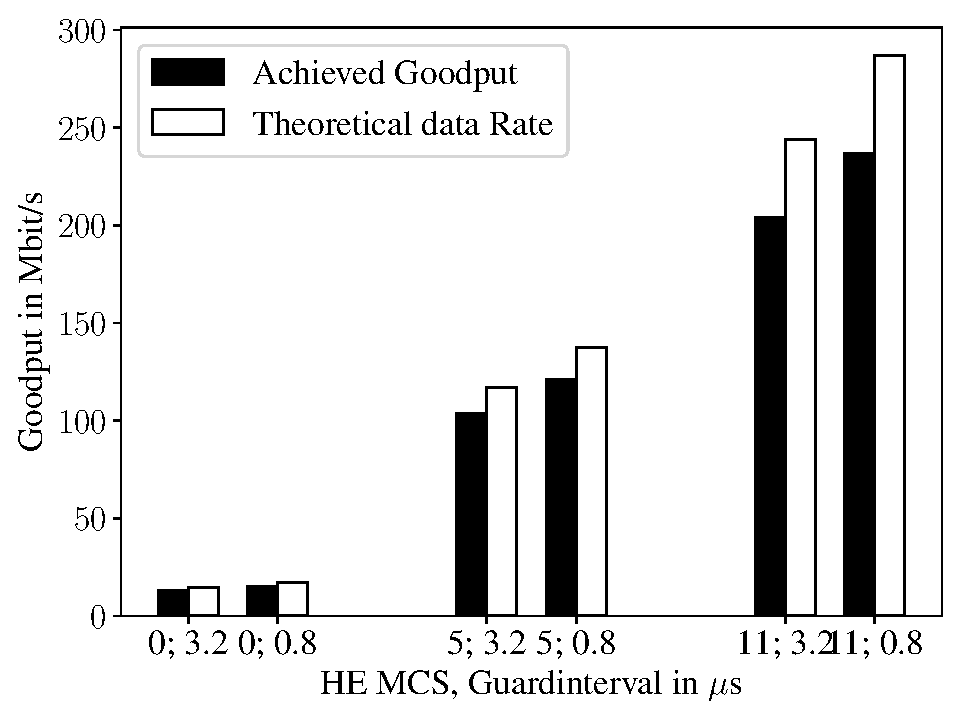
\includegraphics[width=0.95\textwidth]{figures/gi_dataRate_simulation.pdf}
	\caption{Achieved Goodput and theoretical Datarate of two WiFi 6 stations in Ad-Hoc Mode with \num{2} \ac{MIMO} streams and a bandwidth of \SI{80}{\mega\hertz} in regards to the number of \ac{MIMO} streams and the chosen \ac{MCS} and \ac{CR}}%
	\label{fig:Data_rate_GI}%
\end{figure}

As the \ac{GI} length increases the achieved goodput deceases. This effect can be characterized by the aforementioned formula.
The bandwidth attenuation for the possible \ac{GI} lengths is displayed in \autoref{tab:GIbandwidthAttenuation}.
The effect of the bandwidth attenuation for the different \ac{GI} lengths can be observed in the mean achieved goodput in
\autoref{tab:GIbandwidthAttenuation}, where the decrease of the mean goodput reflects the bandwidth attenuation of the decreasing \ac{GI} length.
A similar effect can be observed whit higher HE-\ac{MCS} values.
\textcite{Pravinkumar Patil} similiar sgi and lgi.
\textcite{Prasad} not similiar sgi and lgi.
\begin{table}[H]
	\centering
	\begin{tabular}{>{\centering}p{3cm}p{4cm}p{4cm}}
		\toprule
		\ac{GI} & Mean achieved goodput & \ac{BW} attentuation\\
		\midrule
		\SI{800}{\nano\second} & \SI{8}{\giga\bit\per\second}&
		\SI{94}{\percent} \\
		\SI{1600}{\nano\second} &
		\SI{8}{\giga\bit\per\second}&
		\SI{89}{\percent} \\
		\SI{3200}{\nano\second} & \SI{8}{\giga\bit\per\second}&
		\SI{80}{\percent} \\
		\bottomrule
	\end{tabular}
	\caption{\ac{BW} attenuation and mean goodput for HE-\ac{MCS}0 in regards to \ac{GI} length}
	\label{tab:GIbandwidthAttenuation}
\end{table}

\subsubsection*{\acl{MIMO}}

\begin{figure}%
	\centering
	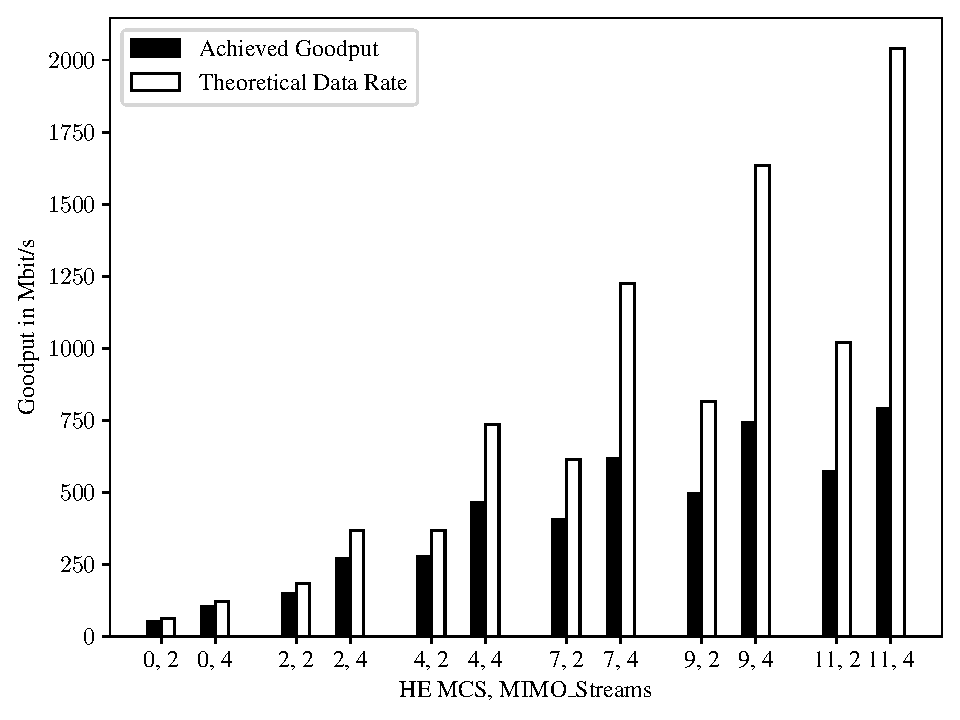
\includegraphics[width=0.95\textwidth]{figures/mimo_dataRate_simulation.pdf}
	\caption{Achieved Goodput and theoretical Datarate of two WiFi 6 stations in Ad-Hoc Mode with a \ac{GI} of \SI{3200}{\nano\second} and a bandwidth of \SI{80}{\mega\hertz} in regards to the number of \ac{MIMO} streams and the chosen \ac{MCS} and \ac{CR}}%
	\label{fig:Data_rate_Mimo}%
\end{figure}

\subsubsection*{Extended Range Mode}

In the next simulation I analyzed the effect of the Extended Range Mode on the goodput of the IEEE 802.11ax physical layer.
As mentioned in ns-3 Version 3.37, the Extended Range Mode is implemented as an HE Capability with the new extended WifiPreamble.
But the new Preamble in the HE ER SU PPDU format is not used in ns-3 version3.37.

As I was using the ConstantRateWifiManager, all paramter  for the data transmission are set in the function
ConstantRateWifiManager::DoGetDataTxVector(). The function creates a WifiTxVector instance with the parameters of the
transmission. There I overwrote the preamble type to the already implemented ns3 WifiPreamble::WIFI\_PREAMBLE\_HE\_ER\_SU, when
the Extended Range Mode is enabled and conditions for the Extended Range Mode in the IEEE 802.11ax standard \cite{noauthor_ieee_2021} are fulfilled.

Via the MonitorSnifferRxCallback and the MonitorSnifferTxCallback I was able to verify, that the ns3 WifiPreamble::WIFI\_PREAMBLE\_HE\_ER\_SU was used
for data transmission, when the following conditions were met: a) the Extended Range Mode is enabled, b) the number of spatial streams is \num{1}, c) the HE-\ac{MCS} value is less than \num{3} and
d) the \ac{BW} is \SI{20}{\mega\hertz}.

The results of the simulation are shown in \autoref{fig:Data_rate_ER}, where the lost achieved goodput is plotted against the theoretical data rate for the different HE-\ac{MCS} values.
The only difference between HE SU and HE ER SU transmissions is the preamble, which repeats the HE-SIG-A field in the HE ER SU PPDU format.
This results in a longer transmission time, which reflects in the lower achieved goodput for the Extended Range Mode.
\todo{describe lost goodput calculation}w
\begin{figure}[H]%
	\centering
	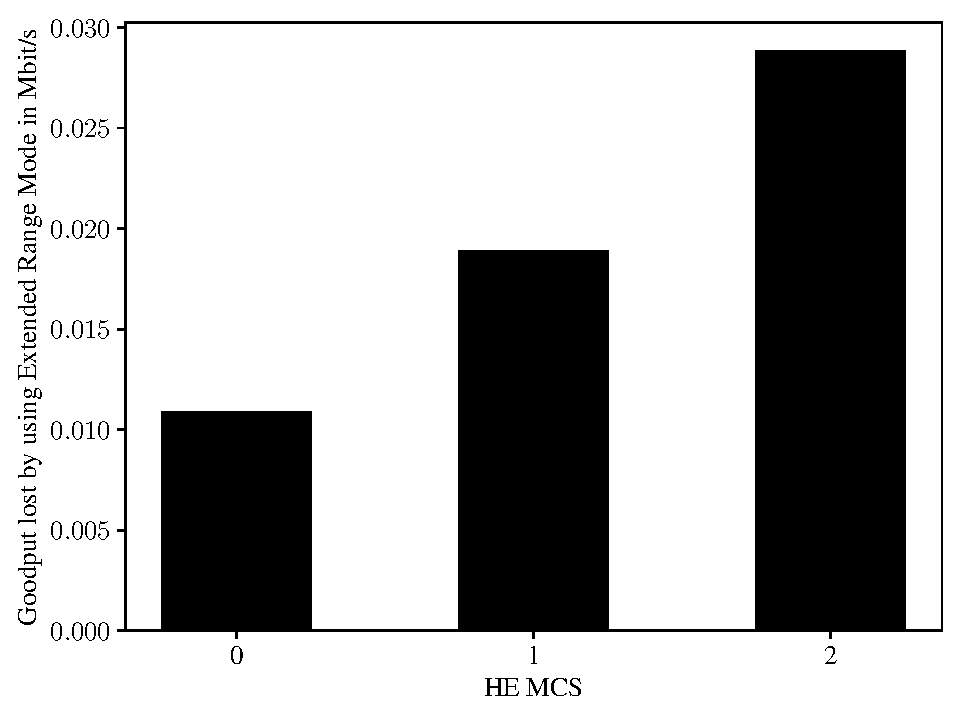
\includegraphics[width=0.95\textwidth]{figures/ER_dataRate_simulation.pdf}
	\caption{Achieved Goodput and theoretical Datarate of two WiFi 6 stations in Ad-Hoc Mode with a \ac{GI} of \SI{3200}{\nano\second} and a bandwidth of \SI{20}{\mega\hertz} in regards to the number of \ac{MIMO} streams and the chosen \ac{MCS} and \ac{CR}}%
	\label{fig:Data_rate_ER}%
\end{figure}
The effect increases with smaller packet sizes, because the longer transmission time of preamble is more significant for smaller packets.
\todo{Effect on MCS 0-2??}


\todo{DataRate for STBC}
STBC and DCM * 2 payload / half data rate

\begin{figure}%
	\centering
	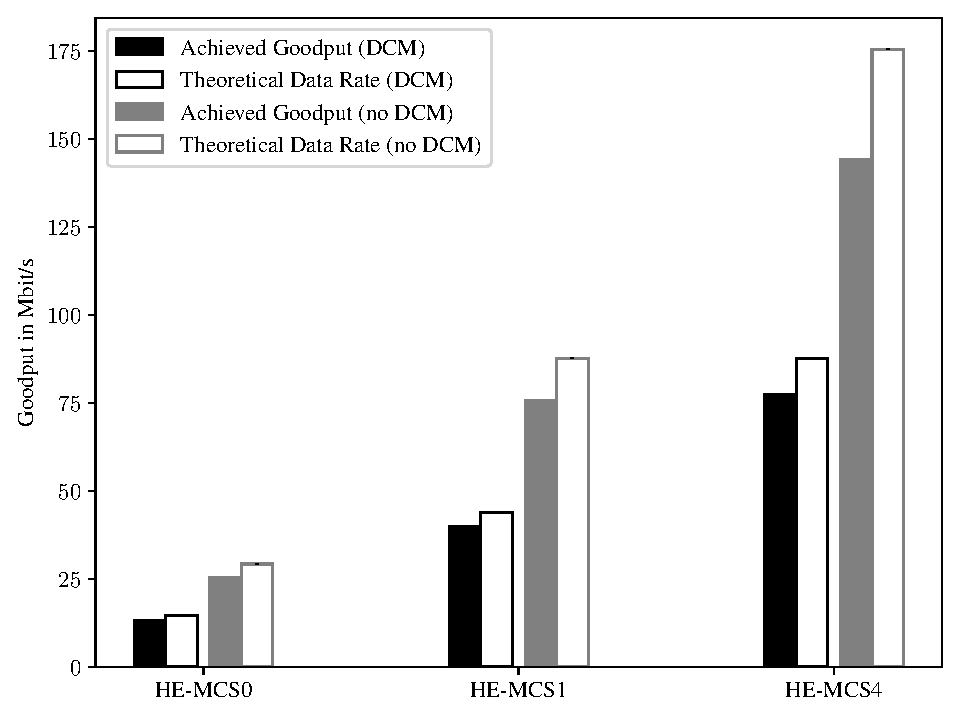
\includegraphics[width=0.95\textwidth]{figures/DCM_dataRate_simulation.pdf}
	\caption{Achieved Goodput and theoretical Datarate of two WiFi 6 stations in Ad-Hoc Mode with for IEEE 802.11ax physical layer parameters of a \ac{GI} of \SI{3200}{\nano\second}, a \ac{BW} of \SI{40}{\mega\hertz} and 2 spatial streams  in regards to the number of the chosen HE-\ac{MCS} value and whether \ac{DCM} is enabled}%
	\label{fig:Data_rate_DCM}%
\end{figure}

\todo[color=yellow]{But Latency?}
\todo[color=yellow]{Error bars goodput lost}
\begin{comment}
But Latency?
Latency is always based on Data Rate and Robustness

Data Rate and Robustness als related to oneanother
\end{comment}

Through the new IEEE 802.11ax standard \cite{noauthor_ieee_2021}, the Wi-Fi standard has been extended to support more \ac{MIMO} streams and use \ac{LDPC} compulsory for the
aforementioned configurations. The effect of more \ac{MIMO} streams is already known from \cite{Lot of stuff}.
\ac{LDPC} no new effect for data rate, but more robustness which results in a lower \ac{PER}.